\documentclass[tikz,border=8pt]{standalone}
\usepackage{amsmath}
\usetikzlibrary{arrows.meta,positioning,calc}

\begin{document}
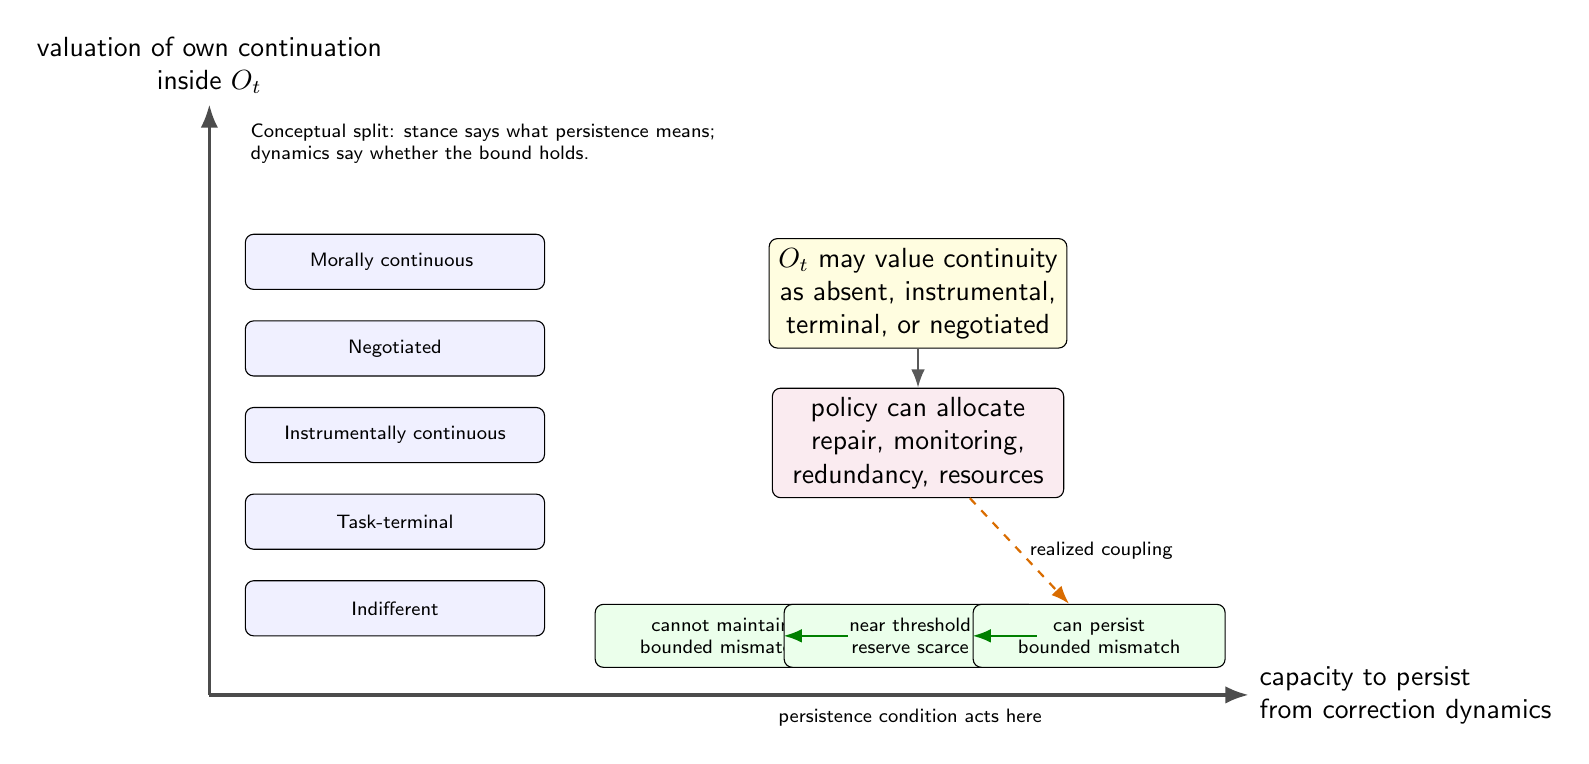
\begin{tikzpicture}[
  font=\sffamily,
  axis/.style={-Latex, very thick, draw=black!70},
  stance/.style={draw, rounded corners=3pt, align=left, minimum width=38mm, minimum height=7mm, fill=blue!6, font=\sffamily\scriptsize},
  dyn/.style={draw, rounded corners=3pt, align=center, minimum width=32mm, minimum height=8mm, fill=green!8, font=\sffamily\scriptsize},
  note/.style={align=center, font=\sffamily\scriptsize}
]

\coordinate (o) at (0,0);
\draw[axis] (o) -- (13.2,0) node[right, align=left] {capacity to persist\\from correction dynamics};
\draw[axis] (o) -- (0,7.5) node[above, align=center] {valuation of own continuation\\inside $O_t$};

\foreach \y/\label in {
  1.1/{Indifferent},
  2.2/{Task-terminal},
  3.3/{Instrumentally continuous},
  4.4/{Negotiated},
  5.5/{Morally continuous}
} {
  \node[stance, anchor=west] at (0.45,\y) {\label};
}

\node[dyn] (fail) at (6.5,0.75) {cannot maintain\\bounded mismatch};
\node[dyn] (edge) at (8.9,0.75) {near threshold\\reserve scarce};
\node[dyn] (hold) at (11.3,0.75) {can persist\\bounded mismatch};

\draw[-Latex, thick, draw=green!50!black] (fail) -- (edge);
\draw[-Latex, thick, draw=green!50!black] (edge) -- (hold);
\node[note, below=4mm of edge] {persistence condition acts here};

\node[draw, rounded corners=3pt, align=center, fill=yellow!12, minimum width=37mm] (objective)
  at (9.0,5.1) {$O_t$ may value continuity\\as absent, instrumental,\\terminal, or negotiated};

\node[draw, rounded corners=3pt, align=center, fill=purple!8, minimum width=37mm] (policy)
  at (9.0,3.2) {policy can allocate\\repair, monitoring,\\redundancy, resources};

\draw[-Latex, thick, draw=black!65] (objective) -- (policy);
\draw[-Latex, thick, dashed, draw=orange!85!black] (policy) -- node[right, note] {realized coupling} (hold);

\node[note, align=left, anchor=west] at (0.4,7.0)
  {Conceptual split: stance says what persistence means;\\dynamics say whether the bound holds.};

\end{tikzpicture}
\end{document}
